\subsection{Motivation}

Les modèles décrits dans ce chapitre ont pour objectif de prédire la longueur de liaison optimisée entre des atomes partageant une liaison covalente au sein d'une molécule. L'objectif n'est donc pas de résoudre le problème de prédiction d'une géométrie moléculaire convergée complète, mais plutôt d'en résoudre une version locale simplifiée. Chronologiquement, cette classe de modèles est apparue après l'abandon des modèles tentant de prédire la géométrie optimisée complète d'une molécule (REF ABANDON DELTA\_DIST).\\
Puisque l'on résout le problème d'optimisation géométrique entre des couples d'atomes, la question de la façon d'utiliser cette méthode pour optimiser la géométrie complète d'une molécule se pose, nous n'y apportons cependant pas de réponse dans ce chapitre. L'objectif de ces modèles est en effet avant tout de valider notre capacité à effectuer des prédictions d'ordre géométrique de précision suffisante sur certains types de liaisons (REF GENERALISATION). L'élaboration d'une méthode d'optimisation géométrique moléculaire complète basée sur la résolution de sous-problèmes locaux est un problème très complexe, qui fait partie des nouveaux objectifs du projet QuChemPedia (REF PERSPECTIVES MODULES).

\subsection{Représentation des données}

\subsubsection{Données en entrée des modèles}
\par Les modèles décrits dans ce chapitre utilisent en entrée la représentation géométrique locale des liaisons covalentes (REF GEOM LOCALE), qui permet de représenter les atomes au voisinage d'une liaison. En plus des informations géométriques, on représente la masse et le numéro atomique de chaque atome au voisinage de la liaison. Le numéro atomique est encodé en \emph{one-hot encoding}, c'est à dire de façon booléenne. La discrétisation des numéros atomiques a pour but de ne pas instaurer de relation d'ordre entre les différents atomes et donc a priori de mieux guider les modèles lors de l'apprentissage. Elle implique toutefois qu'il faut déterminer une limite aux numéros atomiques des atomes acceptés par un modèle. En effet, cet encodage coûte un attribut pour chaque numéro atomique accepté, pour chaque atome au voisinage de la liaison. Afin de travailler sur des modèles de taille raisonnable, ils acceptent les atomes de numéros atomiques inférieurs ou égaux à celui du fluor, ce qui correspond à neuf attributs encodant le numéro atomique pour chaque atome du voisinage.
\par De même la classe positionnelle (REF CLASSE POS) de chaque atome par rapport à la liaison est représenté en \emph{one-hot encoding}, afin de ne pas représenter cette information sur un ensemble possédant une relation d'ordre.\\

\par Le tableau suivant présente le nombre d'attributs utilisés pour représenter chaque atome au voisinage d'une liaison.

\begin{figure}[!h]
	\centering
	
	\begin{tabular}{|c|c|c|c|c|}
		\hline
		\textbf{Classe positionnelle} & \textbf{Distances} & \textbf{Masse atomique} & \textbf{Numéro atomique} & \textbf{Total}\\ \hline
		3 & 2 & 1 & 9 & 15\\ \hline
	\end{tabular}
	\caption{Quantité d'attributs représentant chaque atome au voisinage d'une liaison}
\end{figure}

\subsubsection{Homogénéisation de la taille des entrées}
\par Les molécules possédant un nombre variable d'atomes et l'entrée des modèles étant de taille fixe, nous effectuons une procédure de \emph{padding}\footnote{Rembourrage} des données. Cela signifie que l'entrée des modèles est découpée en blocs, représentant chacun un atome au voisinage de la liaison. La taille des blocs dépend des attributs représentant chaque atome, et le nombre de blocs définit le nombre maximal d'atomes au voisinage des liaisons que les modèles peuvent traiter. Nous déduisons cette information de la taille des molécules que l'on choisit d'accepter en entrée des modèles. La grande majorité des molécules étant de taille inférieure à 60 (VOIR DONNEES DISTRIB TAILLES) et les deux atomes composant la liaison n'apparaissant pas dans les entrées, nous choisissons de limiter le voisinage de la liaison à 58 atomes.\\
\par La représentation d'une liaison en entrée des modèles est donc composée de 58 blocs de 15 attributs, soit 870 valeurs. Lorsqu'une liaison possède moins de 58 voisins, les blocs correspondant aux atomes non définis valent zéro.

\subsubsection{Représentation d'une liaison en entrée d'un modèle}

\par Nous détaillons la représentation en entrée d'un modèle prédictif de la liaison imaginaire utilisée comme exemple en (REF REPR LOCALE). On considère que l'atome a$_3$ est un atome d'azote et que l'atome a$_4$ est un atome d'oxygène.

\vspace{0.5cm}

\begin{figure}[!h]
	\centering
	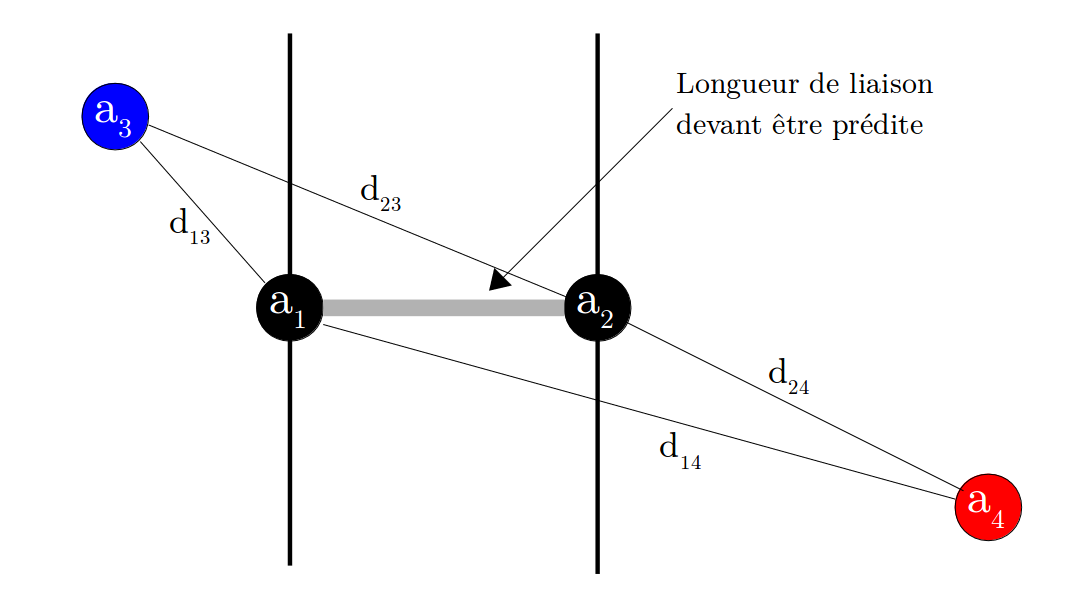
\includegraphics[scale=0.3]{images/classes_pos_4.png}
	\caption{Représentation schématique d'une liaison imaginaire}
\end{figure}

\par L'entrée correspondant à la liaison représentée ci-dessus est donnée dans le tableau suivant.

\begin{figure}[!h]
	\centering


	\begin{tabular}{|c|c|c|c|c|c|c|c|c|c|c|c|c|c|c|}
		\hline
		\multicolumn{3}{|c|}{\textbf{Classe pos.}} & \multicolumn{2}{|c|}{\textbf{Distances}} & \textbf{Masse atomique} & \multicolumn{9}{|c|}{\textbf{Numéro atomique}} \\
		\textbf{g?} & \textbf{c?} & \textbf{d?} & \multicolumn{2}{|c|}{}& & \textbf{H?} & \textbf{He?} & \textbf{Li?} & \textbf{Be?} & \textbf{B? }& \textbf{C?} & \textbf{N?} & \textbf{O?} & \textbf{F?} \\ \hline
		1 & 0 & 0 & $d_{13}$ & $d_{23}$ & 14,007 & 0 & 0 & 0 & 0 & 0 & 0 & 1 & 0 & 0 \\ \hline
		0 & 0 & 1 & $d_{14}$ & $d_{24}$ & 15,999 & 0 & 0 & 0 & 0 & 0 & 0 & 0 & 1 & 0 \\ \hline
		0 & 0 & 0 & 0 & 0 & 0 & 0 & 0 & 0 & 0 & 0 & 0 & 0 & 0 & 0 \\ \hline
		\rot{... } & \rot{... } & \rot{... } & \rot{... } & \rot{... } & \rot{... } & \rot{... } & \rot{... } & \rot{... } & \rot{... } & \rot{... } & \rot{... } & \rot{... } & \rot{... } & \rot{... }  \\ \hline 
		0 & 0 & 0 & 0 & 0 & 0 & 0 & 0 & 0 & 0 & 0 & 0 & 0 & 0 & 0 \\ \hline
	\end{tabular}

	\caption{Représentation des données d'une liaison en entrée d'un modèle prédictif}
\end{figure}



\subsection{Méthodologie}

\subsubsection{Précision requise}
\par Les modèles décrits dans ce chapitre travaillent sur des données « parfaites », c'est à dire qu'il prédisent des longueurs de liaisons dans des molécules dont la géométrie a déjà été optimisée. Cela nous permet de confirmer notre capacité à effectuer des prédictions d'ordre géométrique, mais pas de nous assurer que les modèles pourront effectuer de bonnes prédictions sur des données non optimisées issues de mesures ou de résultats théoriques. L'entraînement de modèles travaillant sur des données imparfaites fera l'objet de la suite du projet QuChemPedia (REF PERSPECTIVES). Pour pouvoir espérer obtenir de bonnes prédictions sur des données non optimisées, il faut obtenir de très bons résultats sur des données optimisées, comme on le montre en REF GENERALISATION.

\par La précision que l'on peut espérer atteindre avec les données sur lesquelles les modèles s'entraînent (REF PUBCHEM) est de l'ordre du picomètre (pm), soit $10^{-12}$ m. Cette précision dépend des fonctions choisies lors de l'optimisation géométrique quantique des molécules (REF OPTI DFT). Les modèles effectuant des prédictions dont l'erreur est inférieure à 1 pm auront donc confirmé notre capacité à effectuer des prédictions d'ordre géométrique de précision suffisante.

\subsubsection{Classes de modèles}
\par Nous tentons de prédire les longueurs de liaisons entre plusieurs couples d'atomes, en entraînant un modèle par couple d'atomes formant une liaison. Les liaisons carbone-carbone ne seront alors pas prédites par le même modèle que les liaisons carbone-hydrogène. Cette séparation en sous-problèmes segmentés a pour objectif d'évaluer la précision que peuvent atteindre les modèles sur les problèmes les plus simples que l'on peut leur donner. L'évaluation de leur précision sur des problèmes plus complexes fait partie des futurs objectifs (REF	MODULES PLUSIEURS LIAISONS). La prédiction des longueurs de liaisons d'un unique couple donné d'atomes par modèle n'en fait toutefois pas un problème trivial, car elles peuvent sensiblement varier en fonction des atomes impliqués (REF DISTRIB LONGUEURS). Si les liaisons oxygène-hydrogène ont une taille variant en général entre 96 pm et 106 pm soit avec une étendue de 10 pm, la taille des liaisons carbone-carbone varie entre 120 pm et 160 pm, ce qui représente une étendue de 40 pm. \\
\par L'entraînement des modèles est un processus qui prend un temps non négligeable (REF CONTRAINTES MATERIELLES). Pour cette raison, nous n'entraînons pas tous les modèles sur un grand nombre d'exemples et nous définissons deux classes de modèles ayant des objectifs différents. \\
\par La première classe de modèles a un objectif d'expérimentation. Les modèles sont entraînés sur un nombre relativement faible d'exemples différents (2770924) sur 150 époques (REF DEF EPOCH), ce qui représente environ 2h de préparation de données et 6h d'entraînement avec le matériel disponible. Ces modèles sont entraînés dans le but d'expérimenter de nouveaux traitements des données d'entrée ou de nouveaux paramètres. Ils ont pour objectif de discriminer la qualité de ces entrées et paramètres, c'est pourquoi ils travaillent sur la prédiction difficile des distances de liaisons carbone-carbone. Ces modèles sont décrits en REF PRED C\\
\par La seconde classe de modèles a un objectif de validation des paramètres performants issus de l'entraînement des modèles de la première classe, ainsi qu'un objectif de généralisation des méthodes à différents types de liaisons. Ces modèles s'entraînent donc sur plus d'exemples et sur plusieurs liaisons différentes (carbone-carbone, carbone-hydrogène et oxygène-hydrogène). L'entraînement des trois modèles de cette classe pour un ensemble d'entrées et de paramètres donné prend environ deux jours. Ces modèles sont décrits en REF GENERALISATION.

\subsection{Nomenclature}
\par Afin d'y faire référence simplement, nous nommons les différents modèles que l'on entraîne. Tous les modèles décrits dans ce chapitre ont pour préfixe \emph{DIST\_REL}, issu de leur vocation à prédire la distance relative entre les atomes d'une liaison, et pour suffixe le numéro chronologique de leur entraînement au sein de leur classe.\\
Les modèles de la première classe (resp. seconde) ont pour préfixe \emph{DIST\_REL\_C} (resp. \emph{DIST\_REL\_XY}, où X et Y désignent les symboles des éléments formant la liaison prédite). La différence de nomenclature entre les deux classes et notamment entre les modèles \emph{DIST\_REL\_C} et \emph{DIST\_REL\_CC} est discutable, mais a pour avantage de faire apparaître simplement la distinction.\\
Enfin, les modèles prédictifs n'étant pas des réseaux de neurones artificiels font apparaître leur type dans leur nom.
